\section{原理}

\subsection{結晶性熱可塑性高分子材料}
熱すると溶けて冷却すると硬化する高分子材料は熱可塑性高分子材料と呼ばれる.熱可塑性高分子材料でも,硬化する際に分子鎖が秩序をもって配列するものがあり,このような材料は結晶性を有するといわれる.ただし,金属材料のような広範囲の規則正しい配列ではなく,図\ref{fig:crystalline}のような分子鎖が折りたたまった構造となっている.この領域を高分子の結晶相とし,それ以外の不規則に分子鎖が絡まり合った領域は非晶相と呼ばれる.また,一部の結晶性高分子材料は図\ref{fig:階層構造}のような結晶相と非晶相が積み重なり,核から放射状に成長することによって形成される球晶と呼ばれる微細組織を形成する.球晶の大きさはおよそ数十~数百μm程度であり,偏光顕微鏡観察によって観察することができる(図\ref{fig:球晶構造}).

\begin{figure}[htbp]
    \begin{minipage}[htbp]{0.45\linewidth}
      \centering
      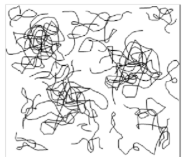
\includegraphics[keepaspectratio, scale=1]{fig/fig_amorphous.png}
      \subcaption{Amorphous polymer}
      \label{fig:amorphous}
    \end{minipage}
    \begin{minipage}[htbp]{0.45\linewidth}
      \centering
      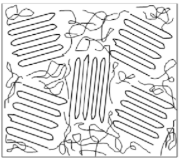
\includegraphics[keepaspectratio, scale=1]{fig/fig_crystalline.png}
      \subcaption{Crystalline polymer}
      \label{fig:crystalline}
    \end{minipage}
    \centering
    \caption{Amorphous and crystalline polymer materialsg.}
    \label{fig:amorphous_crystalline}
\end{figure}

\begin{figure}[htbp]
    \centering %中央揃え
    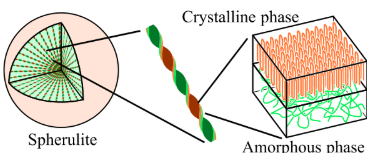
\includegraphics[width=100truemm,clip]{fig/fig_階層構造}
    \caption{Hierarchical structure of spherulite.}
    \label{fig:階層構造}
\end{figure}

\begin{figure}[htbp]
    \centering %中央揃え
    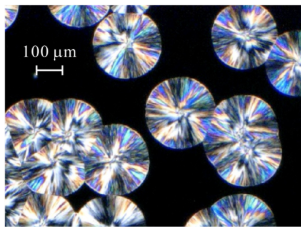
\includegraphics[width=100truemm,clip]{fig/fig_球晶構造}
    \caption{Spherocrystalline structure of polylactic acid.}
    \label{fig:球晶構造}
\end{figure}

\subsection{球晶の形成過程}
球晶が形成される際の核の形成速度$\dot n$と球晶の成長速度$\dot d$は次の式を用いてモデル化されている.ここで$\dot n_0$はエネルギー障壁がないときの核形成速度, $\Delta E_1$は液相中の分子鎖が核になるまでの輸送にかかる運動エネルギー,$R$はBoltzmann定数,$T$は絶対温度,$K_1$は核形成因子パラメータ,$T_m$は完全結晶の融点(平衡融点),はエネルギー障壁がないときの球晶成長速度,$\Delta E_2$は液相中の分子鎖が球晶に組み込まれるまでの輸送にかかる運動エネルギーおよび $K_2$は球晶成長因子パラメータである.式(1),式(2)および実験などから決定される適切なパラメータを用いれば,核形成速度および球晶成長速度が図5のように表される.核形成速度と球晶成長速度が温度によって異なるため,球晶の数や大きさは成形温度に依存する.

\begin{equation}
    \dot n = \dot n_0 \exp \left\{ -\frac{\Delta E_1}{RT} - \frac{K_1 T_m^2}{RT(T_m - T)^2} \right\}
\end{equation}
\begin{equation}
    \dot d = \dot d_0 \exp \left\{ -\frac{\Delta E_2}{RT} - \frac{K_2 T_m^2}{RT(T_m - T)^2} \right\}
\end{equation}

\begin{figure}[htbp]
    \begin{minipage}[htbp]{0.45\linewidth}
      \centering
      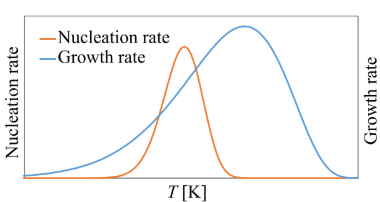
\includegraphics[keepaspectratio, scale=0.7]{fig/fig_模式図.png}
      \subcaption{Schematic diagram}
      \label{fig:模式図}
    \end{minipage}
    \begin{minipage}[htbp]{0.45\linewidth}
      \centering
      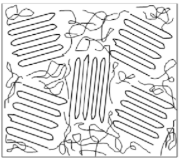
\includegraphics[keepaspectratio, scale=1]{fig/fig_crystalline.png}
      \subcaption{Spherulite growth rate of polypropylene}
      \label{fig:ポリプロピレン成長速度}
    \end{minipage}
    \centering
    \caption{Nucleation rate and spherulite growth rate.}
    \label{fig:核生成速度と成長速度}
\end{figure}